\documentclass{article}

\usepackage{calculator}
\usepackage{calculus}

\usepackage{fancyhdr}
\usepackage{extramarks}
\usepackage{amsmath}
\usepackage{amsthm}
\usepackage{amsfonts}
\usepackage{tikz}
\usepackage[plain]{algorithm}
\usepackage{algpseudocode}
\usepackage{tikz,pgfplots,multicol}
\usepackage[font=small,labelformat=empty]{caption}
\usetikzlibrary{automata,positioning,arrows,patterns}
\usepackage{enumitem}

%
% Basic Document Settings
%

\topmargin=-0.45in
\evensidemargin=0in
\oddsidemargin=0in
\textwidth=6.5in
\textheight=9.0in
\headsep=0.25in

\linespread{1.1}

\pagestyle{fancy}
\lhead{\hmwkAuthorName}
\chead{\hmwkClass\ (\hmwkClassInstructor\ \hmwkClassTime)}
\rhead{\hmwkTitle}
\lfoot{\lastxmark}
\cfoot{\thepage}

\renewcommand\headrulewidth{0.4pt}
\renewcommand\footrulewidth{0.4pt}

\setlength\parindent{0pt}

\setcounter{secnumdepth}{0}
\newcounter{partCounter}
\newcounter{homeworkProblemCounter}
\setcounter{homeworkProblemCounter}{1}
\nobreak\extramarks{Problem \arabic{homeworkProblemCounter}}{}\nobreak{}

%
% Homework Problem Environment
%
% This environment takes an optional argument. When given, it will adjust the
% problem counter. This is useful for when the problems given for your
% assignment aren't sequential. See the last 3 problems of this template for an
% example.
%
\newenvironment{homeworkProblem}[1][-1]{
    \ifnum#1>0
        \setcounter{homeworkProblemCounter}{#1}
    \fi
    \section{Problem \arabic{homeworkProblemCounter}}
    \setcounter{partCounter}{1}
    \enterProblemHeader{homeworkProblemCounter}
}{
    \exitProblemHeader{homeworkProblemCounter}
}

%
% Homework Details
%   - Title
%   - Due date
%   - Class
%   - Section/Time
%   - Instructor
%   - Author
%

\newcommand{\hmwkTitle}{HW \#10}
\newcommand{\hmwkDueDate}{March 23, 2017}
\newcommand{\hmwkClass}{MATH 1300}
\newcommand{\hmwkClassTime}{Section 005}
\newcommand{\hmwkClassInstructor}{Professor Braden Balentine}
\newcommand{\hmwkAuthorName}{\textbf{John Keller}}

%
% Title Page
%

\title{
    \vspace{2in}
    \textmd{\textbf{\hmwkClass:\ \hmwkTitle}}\\
    \normalsize\vspace{0.1in}\small{Due\ on\ \hmwkDueDate\ at 10:00am}\\
    \vspace{0.1in}\large{\textit{\hmwkClassInstructor\ \hmwkClassTime}}
    \vspace{3in}
}

\author{\hmwkAuthorName}
\date{}

\renewcommand{\part}[1]{\textbf{\large Part \Alph{partCounter}}\stepcounter{partCounter}\\}

%
% Various Helper Commands
%

% Useful for algorithms
\newcommand{\alg}[1]{\textsc{\bfseries \footnotesize #1}}

% For derivatives
\newcommand{\deriv}[1]{\frac{\mathrm{d}}{\mathrm{d}x} (#1)}

% For partial derivatives
\newcommand{\pderiv}[2]{\frac{\partial}{\partial #1} (#2)}

% Integral dx
\newcommand{\dx}{\mathrm{d}x}

% Alias for the Solution section header
\newcommand{\solution}{\textbf{\large Solution}}

% Probability commands: Expectation, Variance, Covariance, Bias
\newcommand{\E}{\mathrm{E}}
\newcommand{\Var}{\mathrm{Var}}
\newcommand{\Cov}{\mathrm{Cov}}
\newcommand{\Bias}{\mathrm{Bias}}


\usepackage{xcolor}
    \colorlet{Curve}{red!75!black}
    \colorlet{Tangent}{blue!75!black}
\usepackage{pgfplots}
    \pgfplotsset{compat=1.10}
    \usetikzlibrary{
        calc,
        intersections,
        math,
    }
    \makeatletter
        \def\parsenode[#1]#2\pgf@nil{%
            \tikzset{label node/.style={#1}}
            \def\nodetext{#2}
        }
        \tikzset{
            % define style for the points
            Point/.style={
                shape=circle,
                inner sep=0pt,
                minimum size=3pt,
            },
            add node at x/.style 2 args={
                name path global=plot line,
                /pgfplots/execute at end plot visualization/.append={
                        \begingroup
                        \@ifnextchar[{\parsenode}{\parsenode[]}#2\pgf@nil
                    \path [name path global = position line #1-1]
                        ({axis cs:#1,0}|-{rel axis cs:0,0}) --
                        ({axis cs:#1,0}|-{rel axis cs:0,1});
                    \path [xshift=1pt, name path global = position line #1-2]
                        ({axis cs:#1,0}|-{rel axis cs:0,0}) --
                        ({axis cs:#1,0}|-{rel axis cs:0,1});
                    \path [
                        name intersections={
                            of={plot line and position line #1-1},
                            name=left intersection
                        },
                        name intersections={
                            of={plot line and position line #1-2},
                            name=right intersection
                        },
                        label node/.append style={pos=1}
                    ] (left intersection-1) -- (right intersection-1)
                        node [label node]{\nodetext};
                    % ---------------------------------------------------------
                    % draw the tangent line from a bit right of the point on
                    % the curve to the intersection with the ordinate
                    % and draw the corresponding points
                    \draw [dashed] let
                        \p1=($ (left intersection-1) - (right intersection-1) $),
                        \p2=($ (left intersection-1)!sign(#1)*10mm!(right intersection-1) $),
                        %\p2=($ (left intersection+1) - (right intersection+1) $),
                        \p3=($ ({axis cs:0,0}) - (\p2) $),
                        \n1={\x3/\x1}	% slope of tangent line
                    in
                        (\p2) -- +($ {\n1}*(\x1,\y1) $)
	                        
%                        		node[right,node font=\scriptsize,gray] {$y=$\y1/\x1*sign(#1) $x+$}
%                            node [Point,fill=Tangent] (origin intersection) {}
                            node [Point,fill=Curve] at (left intersection-1) {}
                    ;
                    % ----------
                    % draw the horizontal line at the curve intersection point
                    % plus the label above/below the line
%                    \tikzmath{
%                        coordinate \c1;
%                        \c1=(left intersection-1) - (right intersection-1);
%                        \slope=\cy1/\cx1*sign(#1);
%                        \plusoffset = (#1+1);
%                    }
%                    \pgfmathsetmacro{\AboveBelow}{ \slope>0 ? "above" : "below" }
%                    \draw [dashed]
%                        ([xshift=sign(#1)*2.5mm] left intersection-1) --
%                        (left intersection-1) --
%                            node [\AboveBelow,node font=\scriptsize] {$y=\slope x+\plusoffset$}
%                        (left intersection-1 -| origin intersection) --
%                        +($ sign(#1)*(-2.5mm,0) $)
%                            coordinate [pos=0.5] (a)
%                    ;
%                    % draw the horizontal line at the ordinate intersection point
%                    \draw [dotted] (origin intersection)
%                        +($ sign(#1)*(-2.5mm,0) $) --
%                        (origin intersection);
%                    % draw vertical line left/right of the ordinate
%                    \pgfmathsetmacro{\LeftRight}{ #1<0 ? "right" : "left" }
%                    \draw [stealth-stealth] (origin intersection)
%                        +($ sign(#1)*(-1.25mm,0) $) -- (a)
%                            node [midway,\LeftRight,node font=\scriptsize] {$p$}
%                    ;
%                    % ---------------------------------------------------------
                        \endgroup
                },
            },
        }
    \makeatother
\makeatletter
\def\mathcolor#1#{\@mathcolor{#1}}
\def\@mathcolor#1#2#3{%
  \protect\leavevmode
  \begingroup
    \color#1{#2}#3%
  \endgroup
}
\makeatother


\begin{document}

\maketitle

\pagebreak

\section{Section 4.2}

\begin{enumerate}
\setcounter{enumi}{13}
	\item 
	\begin{enumerate}
		\item Sketch the graph of a function that has two local maxima, one local minimum, and no absolute minimum.
		\begin{center}
		\pgfplotsset{width=13cm,height=7cm, axis equal}
			\begin{tikzpicture}
			\begin{axis}[axis lines=middle,minor y tick num=0,minor x tick num=0,tick style={black},grid style={solid, gray!20}]
				\addplot[domain=-3.4:-3][<-]{tan(deg(x+2.2))+1.31};
				\addplot[color=gray,mark=none,dashed] coordinates { (-3.5,-1.2)(-3.5,1.6)};
				\addplot[domain=-3:1.58, samples=100] {sin(deg(2*x))};
				
				\node[label={90:{local max}},circle,fill,inner sep=1pt] at (axis cs:-2.35,1) {};
				\node[label={270:{local min}},circle,fill,inner sep=1pt] at (axis cs:-0.8,-1) {};
				\node[label={90:{local max}},circle,fill,inner sep=1pt] at (axis cs:0.8,1) {};
				
				\addplot[domain=1.58:2]{-2*x+3.145};
				\addplot[domain=2:3][->]{tan(deg(x-1.8))-1.06};
				\addplot[color=gray,mark=none,dashed] coordinates { (3.2,-1.2)(3.2,1.6)};
			\end{axis}
		\end{tikzpicture}
	\end{center}
		\item Sketch the graph of a function that has three local minima, two local maxima, and seven critical numbers.
	\begin{center}
		\pgfplotsset{width=16cm,height=9cm,ymax=1.2,ymin=-1.2,xmin=-7.1,xmax=8.2}
			\begin{tikzpicture}
			\begin{axis}[axis lines=middle,minor y tick num=0,minor x tick num=0,tick style={black},grid style={solid, gray!20}]
				
				\node[label={90:{critical}},circle,fill,inner sep=1pt] at (axis cs:-5,0) {};
				\node[label={270:{min}},circle,fill,inner sep=1pt] at (axis cs:-2.5,-1.05) {};
				\node[label={90:{critical}},circle,fill,inner sep=1pt] at (axis cs:0,0) {};
				\node[label={90:{max}},circle,fill,inner sep=1pt] at (axis cs:2.31,1) {};
				\node[label={270:{min}},circle,fill,inner sep=1pt] at (axis cs:3.9,-1) {};
				\node[label={90:{max}},circle,fill,inner sep=1pt] at (axis cs:5.46,1) {};
				\node[label={270:{min}},circle,fill,inner sep=1pt] at (axis cs:7.04,-1) {};
				
				\draw [fill=white] (axis cs:8.01,0.375) circle[radius= 0.17 em]; 
%				\node[circle,fill=white] at  {};
				
				\addplot[domain=-7:-3, samples=100][<-] {-(x+5)^3/10};
				\addplot[domain=-3:-2, samples=100] {(x+2.5)^2-1.05};
				\addplot[domain=-2:2, samples=100] {x^3/10};
				\addplot[domain=2:8, samples=100] {sin(deg(2*x-3.07))};

			\end{axis}
		\end{tikzpicture}
	\end{center}
	\end{enumerate}		
\setcounter{enumi}{61}
	\item An object with weight $W$ is dragged along a horizontal plane by a force acting along a rope attached to the object. If the rope makes an angle $\theta$ with the plane, then the magnitude of the force is $$F=\frac{\mu W}{\mu \sin \theta + \cos \theta}$$ where $\mu$ is a positive constant called the \textit{coefficient of friction} and where $0\leq \theta \leq \frac{\pi}{2}$. Show that $F$ is minimized when $\tan \theta = \mu$.
	$$\begin{align}
		F'&=\frac{\mu W(\mu \cos\theta - \sin\theta)}{(\mu \sin \theta + \cos \theta)^2}\\
		0&=\sin\theta - \mu \cos \theta\\
		\mu \cos \theta &= \sin \theta\\
		\mu &= \tan \theta\\
		F(0)&=\frac{\mu W}{\mu \sin 0 + \cos 0}\\
		F(0)&=\mu W\\
		F(\frac{\pi}{2})&= \frac{\mu W}{\mu \sin (\frac{\pi}{2}) + \cos (\frac{\pi}{2})}\\
		F(\frac{\pi}{2})&=\frac{\mu W}{\mu}\\
		F(\frac{\pi}{2})&=W
	\end{align}$$
\setcounter{enumi}{65}
	\item A cubic function is a polynomial of degree 3; that is, it has the form $f(x)=ax^3+bx^2+cx+d$, where $a\neq 0$.
		\begin{enumerate}
			\item Show that a cubic function can have two, one, or no critical number(s). Give examples and sketches to illustrate the three possibilities.
			\begin{itemize}
				\item If $f(x)&=x^3+x^2-x+1$, $f'(x)=3x^2+2x-1$, and since it is zero at $x=\frac{1}{3},-1$, then there are two critical points
				\item If $f(x)&=x^3$, $f'(x)=3x^2$, and since it is zero at $x=0$, then there is one critical point
				\item If $f(x)=x^3+x$, $f'(x)=3x^2+1$, and because $f'(x)$ is never negative, there are no critical points
			\end{itemize}
			
			\item How many local extreme values can a cubic function have?\newline
			A cubic function can have 0 or 2 local extreme values because it must retain the shape of a cubic function, but adding $x^2$ simply puts a small dip in the curve, making it have 2 local extremes.
		\end{enumerate}
\end{enumerate}

\section{Section 4.3}

\begin{enumerate}
	\item Use the graph of $f$ to estimate the values of $c$ that satisfy the conclusion of the Mean Value Theorem for the interval [0,8].
	\begin{center}
		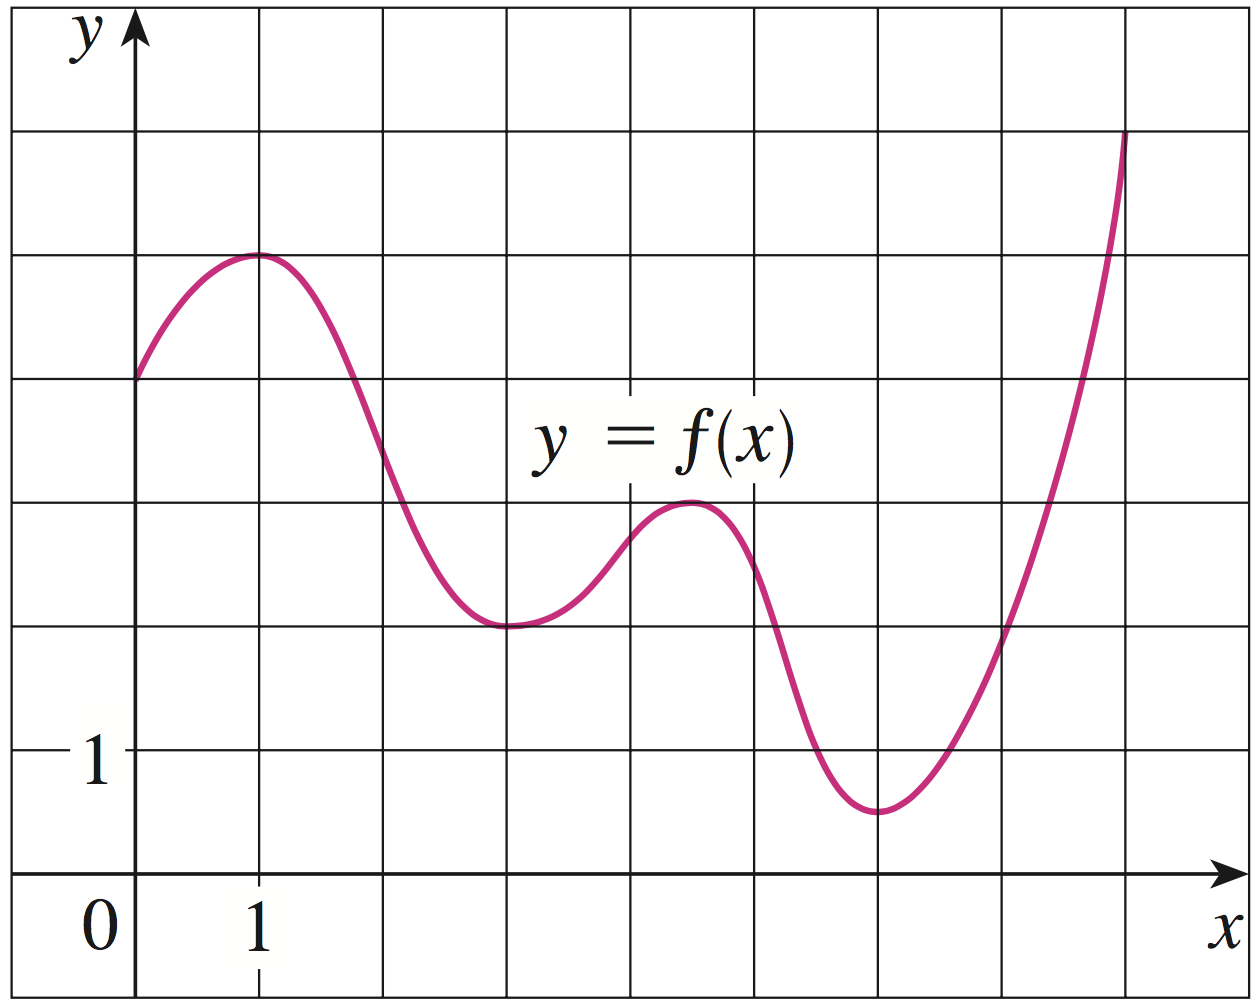
\includegraphics[width=5cm]{images/43pr1.png}
	\end{center}
	$$\begin{align}
		f'(c)&=\frac{f(b)-f(a)}{b-a}\\
		f'(c)&=\frac{6-4}{8-0}\\
		f'(c)&=\frac{2}{8}\\
		f'(c)&=\frac{1}{4}
	\end{align}$$
\setcounter{enumi}{19}
	\item 
		\begin{enumerate}
			\item Find the critical numbers of $f(x)=x^4(x-1)^3$.
			$$\begin{align}
				f'(x)&=-\frac{2x}{(-1+x^2)^2}\\
				0&=(-1+x)^2x^3(-4+7x)\\
				x&=1,0,\frac{4}{7}
			\end{align}$$
			\item What does the Second Derivative Test tell you about the behavior of $f$ at these critical numbers?\newline
			The Second Derivative Test tells us if there is a local maximum or minimum at each critical point.
			\item What does the First Derivative Test tell you?\newline
			The First Derivative Test tells us if there is a local maximum or minimum, as well as if there is neither, at the critical point.
		\end{enumerate}
\setcounter{enumi}{33}
	\item $$f(x)=\frac{x^2}{(x-2)^2}$$
		\begin{enumerate}
			\item Find the vertical and horizontal asymptotes.
			\begin{center}
				\begin{minipage}[t]{0.48\linewidth}
					Finding vertical:
					$$\begin{align}
						0&=(x-2)^2\\
						x&=\boxed{2}
					\end{align}$$
				\end{minipage}
				\begin{minipage}[t]{0.48\linewidth}
					Finding horizontal:
					$$\begin{align}
						\frac{x^2}{x^2}&=\boxed{1} \\
					\end{align}$$
				\end{minipage}
			\end{center}
			\item Find the intervals of increase or decrease.\newline
			$$\begin{align}
				f'(x)&=-\frac{4x}{(x-2)^3}\\
				0&=-\frac{4x}{(x-2)^3}\\
				x&=0
			\end{align}$$
			\begin{center}
				Increase: $(0,2)\qquad$ Decrease: $(-\infty,0)\cup(2,\infty)$
			\end{center}
			
			\item Find the local maximum and minimum values.\newline
				Local max: None $\qquad$ Local min: $(0,0)$
			\item Find the intervals of concavity and the inflection points.\\
				$$\begin{align}
					f''(x)&=\frac{8+8x}{-2^4+x^4}\\
					0&=\frac{8+8x}{-16+x^4}\\
					x&=-1
				\end{align}$$
				Concave up: $(-1,2)\qquad$ Concave down: $(-\infty,1)$ 
			\item Use the information from parts (a)-(d) to sketch the graph of $f$.
	\begin{center}
		\pgfplotsset{width=16cm,height=7cm, axis equal}
			\begin{tikzpicture}
			\begin{axis}[axis lines=middle]
				\addplot[domain=-10:1.5, samples=100][<->]{(x^2)/((x-2)^2)};
				\addplot[domain=3:13, samples=200][<->]{(x^2)/((x-2)^2)};
			\end{axis}
		\end{tikzpicture}
	\end{center}
		\end{enumerate}
\setcounter{enumi}{65}
	\item At 2:00 PM a car's speedometer reads 30 mi/h. At 2:10 PM it reads 50 mi/h. Show that at some time between 2:00 and 2:10 the acceleration is exactly 120 mi/$\text{h}^2$.
	\begin{center}
		\pgfplotsset{width=7cm,height=7cm,ymin=28,xmin=-0.01,xtick={0,0.166666666666667},xticklabels={0,$\frac{1}{6}$},ytick={30,50}}
			\begin{tikzpicture}
			\begin{axis}[axis x line=center, axis y line=left,ylabel near ticks,xlabel near ticks,xlabel={time after 2pm (hrs)},ylabel={speed (mph)}]
				\addplot coordinates { (0,30) (0.166666666666667,50) };
			\end{axis}
		\end{tikzpicture}
	\end{center}
	Determining the slope for the graph above:
	$$\begin{align}
		y&=mx+b\\
		m&=\frac{20}{\frac{1}{6}}
		m&=120x
	\end{align}$$
	As long as $x$ starts at 0 (or 2pm), the acceleration is going to start off at 120 mi/$\text{h}^2$.
	\pagebreak
\setcounter{enumi}{69}
	\item For what values of $c$ does the polynomial $P(x)=x^4+cx^3+x^2$ have two inflection points? One inflection point? None? Illustrate by graphing $P$ for several values of $c$. How does the graph change as $c$ decreases?
	$$\begin{align}
		P'(x)&=4x^3+3cx^2+2x\\
		P''(x)&=12x^2+6cx+2\\
		0&=12x^2+6cx+1\\
		2&=12x^2+6cx\\
		2&=6x(2x+c)\\
		2&=6x\\
		x&=\frac{1}{3}\\
		2&=2x+c\\
		x&=\frac{2-c}{2}\\
		\frac{1}{3}&=\frac{2-c}{2}\\
		\frac{2}{2}&=2-c\\
		c&=2-\frac{2}{3}\\
		c&=\frac{4}{3}
	\end{align}$$
	\begin{center}
		\begin{figure}[!htb]
		\minipage{0.32\textwidth}
	  		\pgfplotsset{width=\linewidth,height=\linewidth,xmin=-2,xmax=4}
				\begin{tikzpicture}
				\begin{axis}[axis lines=middle]
					\addplot[samples=100] {x^4+(-3)*x^3+x^2};
				\end{axis}
			\end{tikzpicture}
		  \caption{$P(x)=x^4+(-3)x^3+x^2$}\label{fig:awesome_image1}
		\endminipage\hfill
		\minipage{0.32\textwidth}
	  		\pgfplotsset{width=\linewidth,height=\linewidth,xmin=-4,xmax=2}
				\begin{tikzpicture}
				\begin{axis}[axis lines=middle]
					\addplot[samples=100] {x^4+4*x^3+x^2};
				\end{axis}
			\end{tikzpicture}
		  \caption{$P(x)=x^4+(4)x^3+x^2$}\label{fig:awesome_image2}
		\endminipage\hfill
		\minipage{0.32\textwidth}%
	  		\pgfplotsset{width=\linewidth,height=\linewidth,xmin=-3,xmax=2}
				\begin{tikzpicture}
				\begin{axis}[axis lines=middle]
					\addplot[samples=100] {x^4+(4/3)*x^3+x^2};
				\end{axis}
			\end{tikzpicture}
		  \caption{$P(x)=x^4+(\frac{4}{3})x^3+x^2$}\label{fig:awesome_image3}
		\endminipage
		\end{figure}

	\end{center}
\end{enumerate}

\section{Additional Problem}
Find the absolute extrema of the function \(f(x)= xe^{- x^2/18}\) on the interval \([-2,4]\). 
$$\begin{align}
	f'(x)&=e^{\frac{-x^2}{18}}(1-\frac{1}{9}x^2)\\
	0&=e^{\frac{-x^2}{18}}\\
	\ln(0)&=\frac{-x^2}{18}\\
	18&=-x^2\\
	x&=\sqrt{-18} \text{ DNE}\\
	0&=1-\frac{1}{9}x^2\\
	x&=\pm 3\\
	f(3)&=3e^{\frac{1}{2}} \text{ relative max}\\
	f(-2)&=-2e^{\frac{2}{9}} \text{ local min}\\
	f(4)&=4e^{\frac{8}{9}} \text{ local max}
\end{align}$$

%
\end{document}